% Options for packages loaded elsewhere
\PassOptionsToPackage{unicode}{hyperref}
\PassOptionsToPackage{hyphens}{url}
%
\documentclass[
]{article}
\usepackage{amsmath,amssymb}
\usepackage{iftex}
\ifPDFTeX
  \usepackage[T1]{fontenc}
  \usepackage[utf8]{inputenc}
  \usepackage{textcomp} % provide euro and other symbols
\else % if luatex or xetex
  \usepackage{unicode-math} % this also loads fontspec
  \defaultfontfeatures{Scale=MatchLowercase}
  \defaultfontfeatures[\rmfamily]{Ligatures=TeX,Scale=1}
\fi
\usepackage{lmodern}
\ifPDFTeX\else
  % xetex/luatex font selection
\fi
% Use upquote if available, for straight quotes in verbatim environments
\IfFileExists{upquote.sty}{\usepackage{upquote}}{}
\IfFileExists{microtype.sty}{% use microtype if available
  \usepackage[]{microtype}
  \UseMicrotypeSet[protrusion]{basicmath} % disable protrusion for tt fonts
}{}
\makeatletter
\@ifundefined{KOMAClassName}{% if non-KOMA class
  \IfFileExists{parskip.sty}{%
    \usepackage{parskip}
  }{% else
    \setlength{\parindent}{0pt}
    \setlength{\parskip}{6pt plus 2pt minus 1pt}}
}{% if KOMA class
  \KOMAoptions{parskip=half}}
\makeatother
\usepackage{xcolor}
\usepackage[margin=1in]{geometry}
\usepackage{color}
\usepackage{fancyvrb}
\newcommand{\VerbBar}{|}
\newcommand{\VERB}{\Verb[commandchars=\\\{\}]}
\DefineVerbatimEnvironment{Highlighting}{Verbatim}{commandchars=\\\{\}}
% Add ',fontsize=\small' for more characters per line
\usepackage{framed}
\definecolor{shadecolor}{RGB}{248,248,248}
\newenvironment{Shaded}{\begin{snugshade}}{\end{snugshade}}
\newcommand{\AlertTok}[1]{\textcolor[rgb]{0.94,0.16,0.16}{#1}}
\newcommand{\AnnotationTok}[1]{\textcolor[rgb]{0.56,0.35,0.01}{\textbf{\textit{#1}}}}
\newcommand{\AttributeTok}[1]{\textcolor[rgb]{0.13,0.29,0.53}{#1}}
\newcommand{\BaseNTok}[1]{\textcolor[rgb]{0.00,0.00,0.81}{#1}}
\newcommand{\BuiltInTok}[1]{#1}
\newcommand{\CharTok}[1]{\textcolor[rgb]{0.31,0.60,0.02}{#1}}
\newcommand{\CommentTok}[1]{\textcolor[rgb]{0.56,0.35,0.01}{\textit{#1}}}
\newcommand{\CommentVarTok}[1]{\textcolor[rgb]{0.56,0.35,0.01}{\textbf{\textit{#1}}}}
\newcommand{\ConstantTok}[1]{\textcolor[rgb]{0.56,0.35,0.01}{#1}}
\newcommand{\ControlFlowTok}[1]{\textcolor[rgb]{0.13,0.29,0.53}{\textbf{#1}}}
\newcommand{\DataTypeTok}[1]{\textcolor[rgb]{0.13,0.29,0.53}{#1}}
\newcommand{\DecValTok}[1]{\textcolor[rgb]{0.00,0.00,0.81}{#1}}
\newcommand{\DocumentationTok}[1]{\textcolor[rgb]{0.56,0.35,0.01}{\textbf{\textit{#1}}}}
\newcommand{\ErrorTok}[1]{\textcolor[rgb]{0.64,0.00,0.00}{\textbf{#1}}}
\newcommand{\ExtensionTok}[1]{#1}
\newcommand{\FloatTok}[1]{\textcolor[rgb]{0.00,0.00,0.81}{#1}}
\newcommand{\FunctionTok}[1]{\textcolor[rgb]{0.13,0.29,0.53}{\textbf{#1}}}
\newcommand{\ImportTok}[1]{#1}
\newcommand{\InformationTok}[1]{\textcolor[rgb]{0.56,0.35,0.01}{\textbf{\textit{#1}}}}
\newcommand{\KeywordTok}[1]{\textcolor[rgb]{0.13,0.29,0.53}{\textbf{#1}}}
\newcommand{\NormalTok}[1]{#1}
\newcommand{\OperatorTok}[1]{\textcolor[rgb]{0.81,0.36,0.00}{\textbf{#1}}}
\newcommand{\OtherTok}[1]{\textcolor[rgb]{0.56,0.35,0.01}{#1}}
\newcommand{\PreprocessorTok}[1]{\textcolor[rgb]{0.56,0.35,0.01}{\textit{#1}}}
\newcommand{\RegionMarkerTok}[1]{#1}
\newcommand{\SpecialCharTok}[1]{\textcolor[rgb]{0.81,0.36,0.00}{\textbf{#1}}}
\newcommand{\SpecialStringTok}[1]{\textcolor[rgb]{0.31,0.60,0.02}{#1}}
\newcommand{\StringTok}[1]{\textcolor[rgb]{0.31,0.60,0.02}{#1}}
\newcommand{\VariableTok}[1]{\textcolor[rgb]{0.00,0.00,0.00}{#1}}
\newcommand{\VerbatimStringTok}[1]{\textcolor[rgb]{0.31,0.60,0.02}{#1}}
\newcommand{\WarningTok}[1]{\textcolor[rgb]{0.56,0.35,0.01}{\textbf{\textit{#1}}}}
\usepackage{graphicx}
\makeatletter
\def\maxwidth{\ifdim\Gin@nat@width>\linewidth\linewidth\else\Gin@nat@width\fi}
\def\maxheight{\ifdim\Gin@nat@height>\textheight\textheight\else\Gin@nat@height\fi}
\makeatother
% Scale images if necessary, so that they will not overflow the page
% margins by default, and it is still possible to overwrite the defaults
% using explicit options in \includegraphics[width, height, ...]{}
\setkeys{Gin}{width=\maxwidth,height=\maxheight,keepaspectratio}
% Set default figure placement to htbp
\makeatletter
\def\fps@figure{htbp}
\makeatother
\setlength{\emergencystretch}{3em} % prevent overfull lines
\providecommand{\tightlist}{%
  \setlength{\itemsep}{0pt}\setlength{\parskip}{0pt}}
\setcounter{secnumdepth}{-\maxdimen} % remove section numbering
\usepackage{booktabs}
\usepackage{longtable}
\usepackage{array}
\usepackage{multirow}
\usepackage{wrapfig}
\usepackage{float}
\usepackage{colortbl}
\usepackage{pdflscape}
\usepackage{tabu}
\usepackage{threeparttable}
\usepackage{threeparttablex}
\usepackage[normalem]{ulem}
\usepackage{makecell}
\usepackage{xcolor}
\ifLuaTeX
  \usepackage{selnolig}  % disable illegal ligatures
\fi
\usepackage{bookmark}
\IfFileExists{xurl.sty}{\usepackage{xurl}}{} % add URL line breaks if available
\urlstyle{same}
\hypersetup{
  pdftitle={week7HW},
  pdfauthor={Kyle Bosworth},
  hidelinks,
  pdfcreator={LaTeX via pandoc}}

\title{week7HW}
\author{Kyle Bosworth}
\date{2024-10-15}

\begin{document}
\maketitle

{
\setcounter{tocdepth}{2}
\tableofcontents
}
\subsubsection{Load libraries}\label{load-libraries}

\begin{Shaded}
\begin{Highlighting}[]
\FunctionTok{library}\NormalTok{(here)}
\FunctionTok{library}\NormalTok{(tidyverse)}
\FunctionTok{library}\NormalTok{(maps)}
\FunctionTok{library}\NormalTok{(mapdata)}
\FunctionTok{library}\NormalTok{(mapproj)}
\FunctionTok{library}\NormalTok{(ggspatial)}
\FunctionTok{library}\NormalTok{(data.table)}
\FunctionTok{library}\NormalTok{(ggmap)}
\FunctionTok{library}\NormalTok{(kableExtra)}
\FunctionTok{library}\NormalTok{(prettydoc)}
\FunctionTok{library}\NormalTok{(ggspatial)}
\end{Highlighting}
\end{Shaded}

\subsubsection{Read in Data}\label{read-in-data}

\begin{Shaded}
\begin{Highlighting}[]
\NormalTok{BFdata }\OtherTok{\textless{}{-}} \FunctionTok{read.csv}\NormalTok{(}\FunctionTok{here}\NormalTok{(}\StringTok{"week7"}\NormalTok{, }\StringTok{"data"}\NormalTok{, }\StringTok{"bigfoot.csv"}\NormalTok{))}
\FunctionTok{glimpse}\NormalTok{(BFdata)}
\end{Highlighting}
\end{Shaded}

\begin{verbatim}
## Rows: 5,021
## Columns: 28
## $ observed           <chr> "I was canoeing on the Sipsey river in Alabama. It ~
## $ location_details   <chr> "", "East side of Prince William Sound", "Great swa~
## $ county             <chr> "Winston County", "Valdez-Chitina-Whittier County",~
## $ state              <chr> "Alabama", "Alaska", "Rhode Island", "Pennsylvania"~
## $ season             <chr> "Summer", "Fall", "Fall", "Summer", "Spring", "Fall~
## $ title              <chr> "", "", "Report 6496: Bicycling student has night e~
## $ latitude           <dbl> NA, NA, 41.45000, NA, NA, 35.30110, 39.38745, 41.29~
## $ longitude          <dbl> NA, NA, -71.50000, NA, NA, -99.17020, -81.67339, -7~
## $ date               <chr> "", "", "1974-09-20", "", "", "1973-09-28", "1971-0~
## $ number             <dbl> 30680, 1261, 6496, 8000, 703, 9765, 4983, 31940, 56~
## $ classification     <chr> "Class B", "Class A", "Class A", "Class B", "Class ~
## $ geohash            <chr> "", "", "drm5ucxrc0", "", "", "9y32z667yc", "dpjbj6~
## $ temperature_high   <dbl> NA, NA, 78.17, NA, NA, 71.86, NA, 92.24, NA, NA, 74~
## $ temperature_mid    <dbl> NA, NA, 73.425, NA, NA, 61.425, NA, 80.810, NA, NA,~
## $ temperature_low    <dbl> NA, NA, 68.68, NA, NA, 50.99, NA, 69.38, NA, NA, 53~
## $ dew_point          <dbl> NA, NA, 65.72, NA, NA, 51.03, NA, 67.34, 32.55, NA,~
## $ humidity           <dbl> NA, NA, 0.86, NA, NA, 0.79, NA, 0.68, 0.45, NA, 0.7~
## $ cloud_cover        <dbl> NA, NA, 0.86, NA, NA, 0.11, NA, 0.05, 0.00, NA, 0.6~
## $ moon_phase         <dbl> NA, NA, 0.16, NA, NA, 0.07, NA, 0.76, 0.02, NA, 0.1~
## $ precip_intensity   <dbl> NA, NA, 0.0000, NA, NA, NA, NA, 0.0000, 0.0000, NA,~
## $ precip_probability <dbl> NA, NA, 0.00, NA, NA, NA, NA, 0.00, 0.00, NA, 0.70,~
## $ precip_type        <chr> "", "", "", "", "", "rain", "", "", "", "", "rain",~
## $ pressure           <dbl> NA, NA, 1020.61, NA, NA, 1017.26, NA, 1016.80, 1012~
## $ summary            <chr> "", "", "Foggy until afternoon.", "", "", "Partly c~
## $ uv_index           <int> NA, NA, 4, NA, NA, 7, NA, 8, 8, NA, 6, 10, 6, 7, NA~
## $ visibility         <dbl> NA, NA, 2.750, NA, NA, 10.000, NA, 6.922, 8.880, NA~
## $ wind_bearing       <int> NA, NA, 198, NA, NA, 259, NA, 219, 285, NA, 262, 19~
## $ wind_speed         <dbl> NA, NA, 6.92, NA, NA, 8.41, NA, 1.01, 4.01, NA, 0.4~
\end{verbatim}

Get map and define boundaries

\begin{Shaded}
\begin{Highlighting}[]
\CommentTok{\#Defines the request area for North America map tiles}
\NormalTok{north\_america\_bbox}\OtherTok{\textless{}{-}}\FunctionTok{c}\NormalTok{(}\AttributeTok{left =} \SpecialCharTok{{-}}\DecValTok{180}\NormalTok{, }\AttributeTok{bottom =} \DecValTok{15}\NormalTok{, }\AttributeTok{right =} \SpecialCharTok{{-}}\DecValTok{50}\NormalTok{, }\AttributeTok{top =} \DecValTok{75}\NormalTok{)}

\CommentTok{\#Get map}
\NormalTok{north\_america\_map }\OtherTok{\textless{}{-}} \FunctionTok{get\_stadiamap}\NormalTok{(north\_america\_bbox, }\AttributeTok{zoom =} \DecValTok{4}\NormalTok{, }\AttributeTok{maptype =} \StringTok{"stamen\_terrain"}\NormalTok{)}
\end{Highlighting}
\end{Shaded}

\section{Bigfoot Sightings}\label{bigfoot-sightings}

\begin{Shaded}
\begin{Highlighting}[]
\FunctionTok{ggmap}\NormalTok{(north\_america\_map) }\SpecialCharTok{+}
  \FunctionTok{geom\_point}\NormalTok{(}\AttributeTok{data =}\NormalTok{ BFdata, }\FunctionTok{aes}\NormalTok{(}\AttributeTok{x =}\NormalTok{ longitude, }
                                \AttributeTok{y =}\NormalTok{ latitude,}
                                \AttributeTok{color =}\NormalTok{ season), }\AttributeTok{alpha =} \FloatTok{0.7}\NormalTok{, }\AttributeTok{size =} \DecValTok{2}\NormalTok{)}\SpecialCharTok{+}
  \FunctionTok{scale\_color\_viridis\_d}\NormalTok{(}\AttributeTok{name =} \StringTok{"Season"}\NormalTok{)}\SpecialCharTok{+}
  \FunctionTok{labs}\NormalTok{(}\AttributeTok{title =} \StringTok{"Bigfoot Sighting in North America"}\NormalTok{,}
       \AttributeTok{subtitle =} \StringTok{"Colored by Season"}\NormalTok{,}
       \AttributeTok{x =} \StringTok{"Longitude"}\NormalTok{,}
       \AttributeTok{Y =} \StringTok{"Latitude"}\NormalTok{)}\SpecialCharTok{+}
  \FunctionTok{theme\_minimal}\NormalTok{()}\SpecialCharTok{+}
  \FunctionTok{theme}\NormalTok{(}\AttributeTok{legend.position =} \StringTok{"right"}\NormalTok{,}
        \AttributeTok{plot.title =} \FunctionTok{element\_text}\NormalTok{(}\AttributeTok{size =} \DecValTok{16}\NormalTok{,}
                                  \AttributeTok{face =} \StringTok{"bold"}\NormalTok{),}
        \AttributeTok{plot.subtitle =} \FunctionTok{element\_text}\NormalTok{(}\AttributeTok{size =} \DecValTok{12}\NormalTok{,}
                                     \AttributeTok{face =} \StringTok{"italic"}\NormalTok{),}
        \AttributeTok{panel.grid.major =} \FunctionTok{element\_line}\NormalTok{(}\AttributeTok{color =} \StringTok{"white"}\NormalTok{, }
                                        \AttributeTok{linetype =} \StringTok{"dashed"}\NormalTok{),}
        \AttributeTok{panel.border =} \FunctionTok{element\_rect}\NormalTok{(}\AttributeTok{color =} \StringTok{"black"}\NormalTok{,}
                                    \AttributeTok{fill =} \ConstantTok{NA}\NormalTok{, }
                                    \AttributeTok{size =} \DecValTok{1}\NormalTok{),}
    \AttributeTok{axis.ticks =} \FunctionTok{element\_line}\NormalTok{(}\AttributeTok{size =} \FloatTok{0.5}\NormalTok{), }\CommentTok{\#adding lat and long ticks on the scales}
    \AttributeTok{axis.ticks.length =} \FunctionTok{unit}\NormalTok{(}\FloatTok{0.25}\NormalTok{, }\StringTok{"cm"}\NormalTok{)) }\SpecialCharTok{+}
  \FunctionTok{coord\_cartesian}\NormalTok{(}\AttributeTok{xlim =} \FunctionTok{c}\NormalTok{(}\SpecialCharTok{{-}}\DecValTok{180}\NormalTok{, }\SpecialCharTok{{-}}\DecValTok{50}\NormalTok{), }
                  \AttributeTok{ylim =} \FunctionTok{c}\NormalTok{(}\DecValTok{15}\NormalTok{, }\DecValTok{75}\NormalTok{), }\AttributeTok{expand =} \ConstantTok{FALSE}\NormalTok{)}
\end{Highlighting}
\end{Shaded}

\begin{center}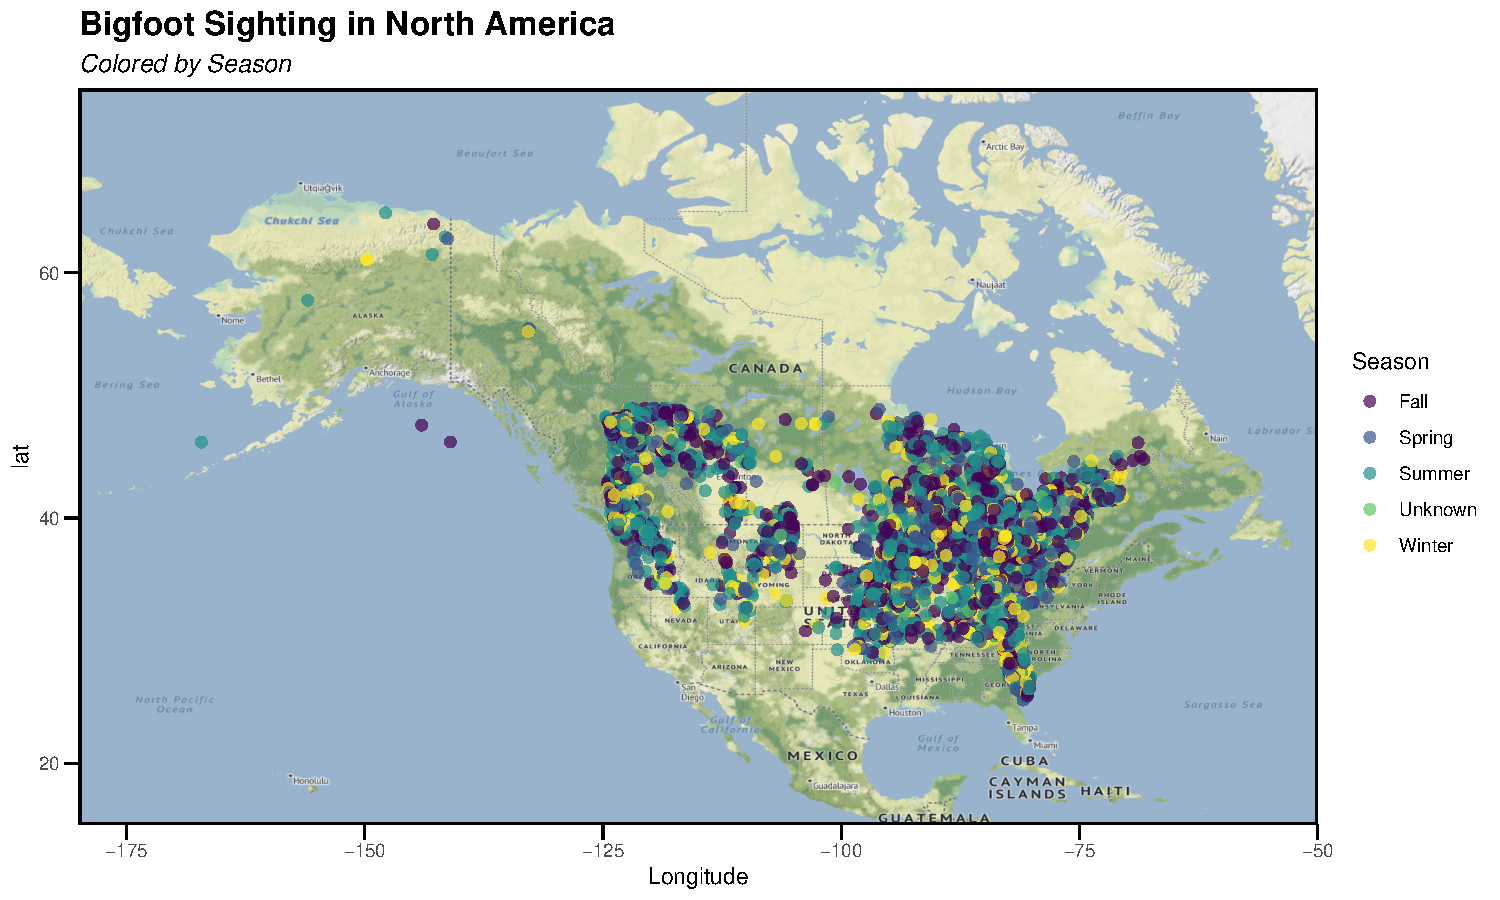
\includegraphics[width=1\linewidth]{week7HW_files/figure-latex/unnamed-chunk-4-1} \end{center}

\end{document}
